\section{Beam Control}
{{\footnotesize
\begin{description}[labelwidth=5em, labelsep=1em, leftmargin=*, align=left, itemsep=0.3em, parsep=0em]
  \item[date:] 2024-05-01
  \item[version:] TODO
  \item[last\_updated:] 2024-05
  \item[expired:] unknown
  \item[valid:] yes
  \item[valid\_date:] TODO
  \item[url:] \href{https://github.com/fastmachinelearning/fastml-science/tree/main/beam-control}{https://github.com/fastmachinelearning/fastml-science/tree/main/beam-control}
  \item[doi:] TODO
  \item[domain:] Accelerators and Magnets
  \item[focus:] Reinforcement learning control of accelerator beam position
  \item[keywords:]
    - RL
    - beam stabilization
    - control systems
    - simulation
  \item[summary:] Beam Control explores real-time reinforcement learning strategies for maintaining 
stable beam trajectories in particle accelerators. The benchmark is based on the 
BOOSTR environment for accelerator simulation.

  \item[licensing:] TODO
  \item[task\_types:]
    - Control
  \item[ai\_capability\_measured:]
    - Policy performance in simulated accelerator control
  \item[metrics:]
    - Stability
    - Control loss
  \item[models:]
    - DDPG
    - PPO (planned)
  \item[ml\_motif:]
    - Real-time, RL
  \item[type:] Benchmark
  \item[ml\_task:]
    - Reinforcement Learning
  \item[solutions:] TODO
  \item[notes:] Environment defined, baseline RL implementation is in progress

  \item[contact.name:] Ben Hawks, Nhan Tran
  \item[contact.email:] unknown
  \item[results.links.name:] ChatGPT LLM
  \item[fair.reproducible:] in progress
  \item[fair.benchmark\_ready:] in progress
  \item[ratings.software.rating:] 0
  \item[ratings.software.reason:] Not analyzed. 

  \item[ratings.specification.rating:] 9.0
  \item[ratings.specification.reason:] Task is well defined (real-time compression of sparse, irregular sensor data using autoencoders); latency constraints are implied but not fully quantified.

  \item[ratings.dataset.rating:] 8.0
  \item[ratings.dataset.reason:] Dataset is custom and synthetic but described well; FAIR-compliance is partial (reusable and accessible, but not externally versioned with rich metadata).

  \item[ratings.metrics.rating:] 9.0
  \item[ratings.metrics.reason:] Uses standard quantitative metrics (MSE, compression ratio) clearly aligned with compression and reconstruction goals.

  \item[ratings.reference\_solution.rating:] 7.0
  \item[ratings.reference\_solution.reason:] Baseline (autoencoder and quantized variant) is provided, but training/inference pipeline is minimally documented and needs user setup.

  \item[ratings.documentation.rating:] 8.0
  \item[ratings.documentation.reason:] GitHub repo contains core components, but more structured setup instructions and pretrained weights would improve usability.

  \item[id:] beam\_control
  \item[Citations:] \cite{duarte2022fastmlsciencebenchmarksaccelerating}, \cite{kafkes2021boostrdatasetacceleratorcontrol}
  \item[Ratings:]
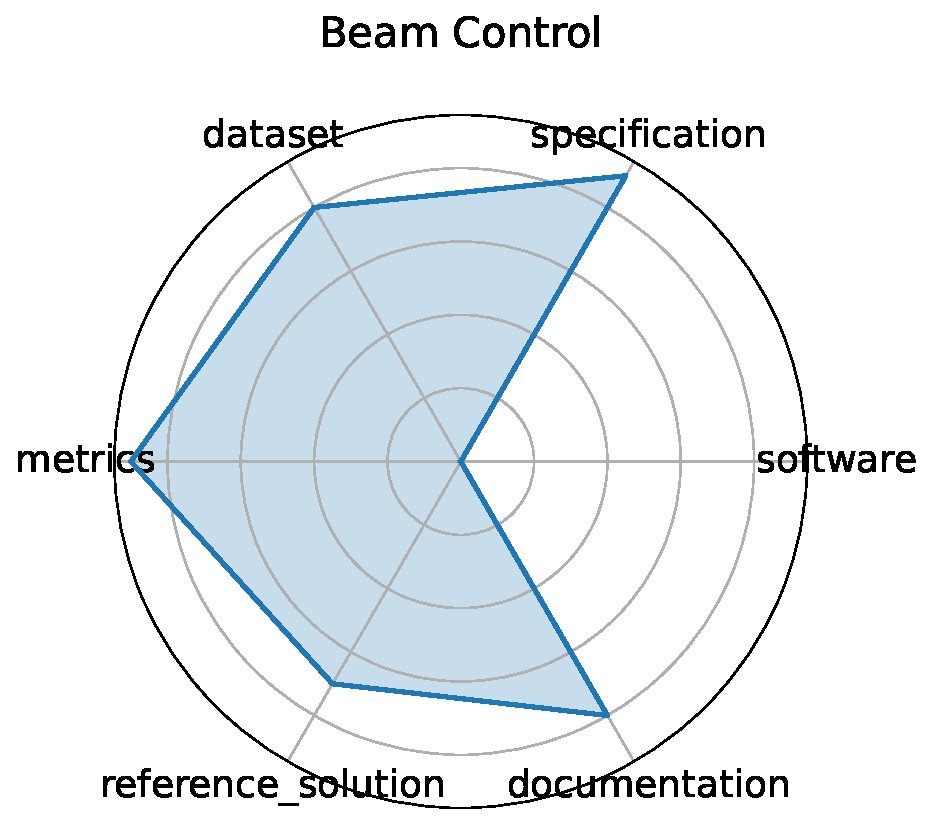
\includegraphics[width=0.2\textwidth]{beam_control_radar.pdf}
\end{description}
}}
\clearpage